\onecolumn
\section*{Appendix A: Data Collection Instructions}
\renewcommand\thefigure{\arabic{figure}}    
\setcounter{figure}{0}   

\begin{tcolorbox}[width=\textwidth,colback={white},title={Rewrite each question in a dialogue so it can be understood by itself without looking at the rest of the dialogue.},colbacktitle=white,coltitle=black]    

\begin{itemize}


\item In the given conversation between a student who asks questions about a topic of a Wikipedia
 article and a teacher who is answering the questions, each question can be understood as part of the
  ongoing dialogue. Edit each question so that it makes sense by itself without looking at the rest of 
   the  dialogue. Think how you would ask the same question to someone who has no idea about what
   the dialogue is about and has never seen any of the previous utterances and still get the same
    answer.
   For example, the question `What was he like in that episode?' cannot be understood without knowing
    what `he' and `that episode' refer to. Both can be figured out by looking at the dialogue. If we edited
    the question to `What was Daffy Duck like in Porky's Duck Hunt?', it would then make sense by
     itself.
     \item Reading and understanding all previous utterances is very important. Do not just look for things
 like `she' and `that' and replace them. For example, the question Who was the star? is still unclear. We
  need to specify `star in what movie, series, episode, ..etc.?' as in Who was the star in Porky's Duck
   Hunt?. To make sure the edits are based on understanding the conversations rather than naive
    replacements, we will manually review a random group of the edits before accepting the work. We
     also run pretty mild checks on the edits before allowing the HIT to be submitted. The checks are
      meant to help you make valid edits, but they still can miss some invalid edits (rather than being too
       strict). So, do not count only on passing the checks and make sure that each edit makes sense by
        itself.

\item Questions should stay in a natural-sounding english after editing. Do not use new words other
 than those in the conversation unless it is necessary. Copy from previous questions, answers and
  conversation topic as often as possible. Never use any information provided after a question is
   asked. Only use what was provided up to the question you are editing. When editing a question,
    keep its original structure whenever possible. For example, do not change `Did they arrest him?' to
     `Was Alex arrested?', but rather keep the original structure and do `Did they arrest Alex?'. Do not
      come up with a different or better question. Stick to the given wording. It is okay to have pronouns
       in an edit as long as the edit has enough information about what the pronouns refer to. For
        example `Where was Carroll when she joined the american party?' is a perfectly fine edit.
        \item Pay special attention to questions that ask if there is anything/anyone else or asking for telling
 more about something. It is important to mention in your edit ``anything/anyone else besides what/
 whom''. For example, `Are there any other interesting aspects about this article?' should be edited to
  something like `Besides Death of a Ladies Man and End of the Century, are there any other
   interesting aspects about this article?' as in example 2 below. Notice that it is okay to keep `this
    article' without replacing it with something else.
    \item If a question can be understood without looking at the rest of the conversation, mark it as
 Understandable alone. Do not make unnecessary edits. Try to keep the edits short as long as they
  make sense each by itself. Although typos are quite rare, please fix any typos you encounter.
  \item Never look up additional information on the web. Only use the given conversations.
\item We show one question at a time. After editing or marking a question as Understandable alone,
 we show its following question. After all questions are edited, we allow you to submit the HIT and
  optionally provide any feedback you have on the HIT.

\end{itemize}
\end{tcolorbox}    

\newpage
\section*{Appendix B: Data Collection Interface}
\begin{figure}[h!]
	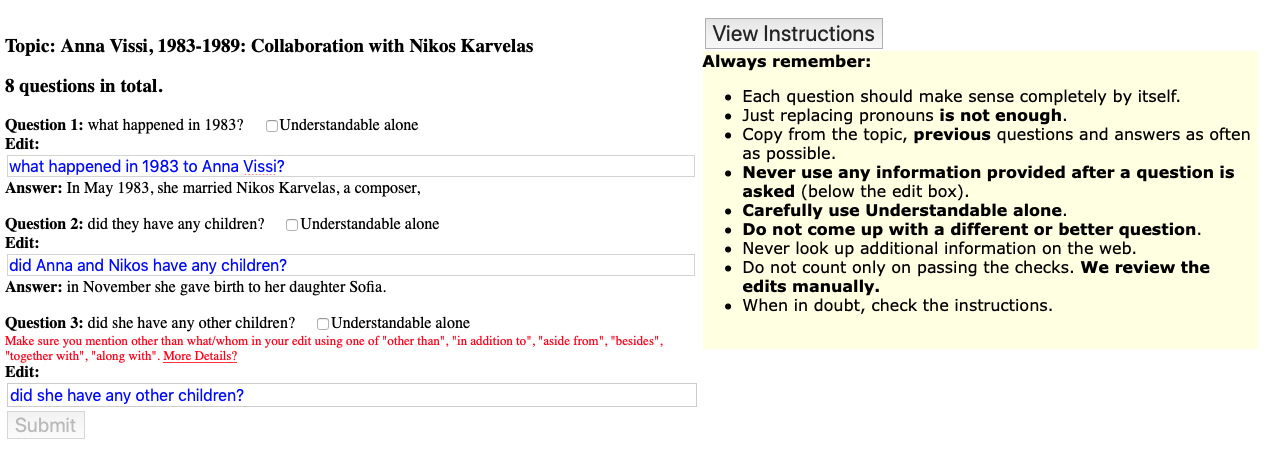
\includegraphics[width=\linewidth]{2019_emnlp_sequentialqa/figures/interface.png}

	\caption{Data collection interface. The conversation has eight questions in total. We show one question at a time
	to encourage crowdworkers only use the \textit{previous} utterances for the rewriting. After the eight questions are
	rewritten, we enable submitting the \abr{hit}. We show question-specific instructions as in question three to remind
	crowdworkers about relevant instructions. A compact set of the full instructions are shown on the right. Detailed
	instructions can be displayed by clicking on the ``view instructions'' button.}
	\label{fig:example_convo}
\end{figure}
